\resizebox{\textwidth}{!}{
	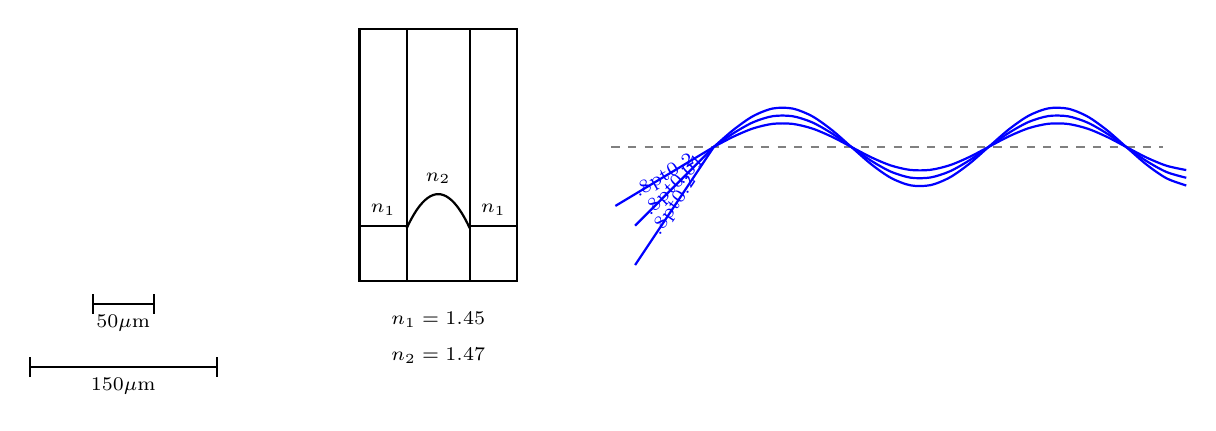
\begin{tikzpicture}[thick, every node/.style={sloped,allow upside down}, font=\scriptsize]
		\begin{scope}[yshift=1.2cm, rotate=-90]
			\doubleCylinder{.6}{.2}{3}
		\end{scope}
		\draw [|-|] (-.4, -2) -- node[below] {50$\mu$m} ++(.8, 0);

		\draw [|-|] (-1.2, -2.8) -- node[below] {150$\mu$m} ++(2.4, 0);

		\begin{scope}[xshift=4cm]
			\draw (-1, -1.7) rectangle (1, 1.5);
			\draw (-.4, -1.7) rectangle (.4, 1.5);

			\draw (-1, -1) -- (-.4, -1);
			\draw (.4, -1) -- (1, -1);
			\draw [smooth, domain=-.4:.4] plot (\x, {-\x*\x*2.7-.6});

			\node at (0, -.4) {$n_2$};
			\node at (-.7, -.8) {$n_1$};
			\node at (.7, -.8) {$n_1$};

			\node at (0, -2.2) {$n_1=1.45$};
			\node at (0, -2.65) {$n_2=1.47$};

			\begin{scope}[xshift=3.5cm]
				\draw [dashed, gray] (-1.3,0) -- ++(7, 0);
				\draw[scale=.5, domain=0:12, smooth, blue] (-2,-3) -- node {\smallmidarrow{.8pt}{0.2}} (0, 0) plot (\x, {sin(\x * .9 r)});
				\draw[scale=.5, domain=0:12, smooth, blue] (-2,-2) -- node {\smallmidarrow{.8pt}{0.01}} (0, 0) plot (\x, {.8*sin(\x * .9 r)});
				\draw[scale=.5, domain=0:12, smooth, blue] (-2.5,-1.5) -- node {\smallmidarrow{.8pt}{0.2}} (0, 0) plot (\x, {.6*sin(\x * .9 r)});
				\doubleCylinder{.7}{.3}{6}
			\end{scope}
		\end{scope}
	\end{tikzpicture}
}